\chapter{Discussion}

We wish to compare the two-dimensional (2D) GLCM method to the three-dimensional (3D), to see if one performs better. To make this comparison we have on our data of 100 patients extracted four data sets for left hippocampus. Data set one, D$_1$, we performed erosion before calculating the GLCMs which are normalized, both are done for the 2D and 3D methods. Data set two, D$_2$, is the same as D$_1$ except no erosion has been performed. Data set three, D$_3$, is with erosion, but no normalizing. Data set four, D$_4$, is without erosion and normalizing.
We also wish to determine which of the left or right hippocampus is best suited to diagnose AD, if there is a difference. Data sets D$_5$, D$_6$, D$_7$, D$_8$ are created as D$_{1-4}$ but on the right hippocampus. \fixme[inline]{Create a table to show what each data set contains?}
Lastly we wish to determine if we can correctly diagnose AD with an accuracy higher than 80\%.



%
%In this paper when calculating the GLCMs we have chosen to work with offsets similar to those used in the paper by Peter A. Freeborough and Nick C. Fox \cite{MRfreeborough} in contrast to the radius method used by Rouzbeh Maani, Yee Hong Yang, Sanjay Kalra \cite{Voxel}.
%The reason we chose to work with offsets is because we wished to compare our results with \cite{MRfreeborough}


The advantage with using offsets compared to the radius computational wise is that despite an increase in distance the amount of angles does not increase, the amount of GLCMs to calculate are No. of offsets $\times$ distances, where as if we were to take the radius the No. of offsets at a given distance, increases with the distance, even when we take into account that we can ignore half of the angles. For  the radius the No. of GLCMs to calculate at distance d is equal to $\sigma_{i=1}^d$3$\cdot$i + 1. So for each additional distance one would have to calculate 3*d+1 additional GLCMS if we were using the radius, compared to just the four offsets. These calculations are just for the two-dimensional, where as in three dimensions this problem is amplified, as each increase in distance increases the number of GLCMS by $\frac{1}{2}$((2d+1)$^3$-1). However as this clearly demonstrates the radius method would gather a lot more information, but considering that we have over a thousand features for each patients, we are not in need of more information. In addition the subject of this paper is inspired by the paper from Peter A. Freeborough and Nick C. Fox \cite{MRfreeborough}, so we are keeping our method similar to theirs, so it  is possible to compare the results.

\section{GOD SECTION TITEL}
In the previous chapter we saw the plots of our data, which are early AD patient, more specific 24-month follow-ups and controle. As our data consists of early AD patients, it can be very difficult to differentiate one from another and thus make it challenging to get some good results, specially if we are to select some features to do machine learning. But luckily we can lean on our algorithm to select features better than we can. In consideration of that we have to feature selection method, the first one is naive selection and the second one is Sequential Feature Selection.\fxnote[inline]{Skriv at vi kun kigger på 3d/2d normalized erode}

\subsection{Naive Selection}
As described previously, often there is no clear visual difference in the plots of the GLCM features, which makes it hard to make a naive selections. This forces us to look after some kind of relationship in the slope, if the data increases or decreases from a distance to another or if either AD or control have a steep slope where the other would have a straight slope. We have chosen to only select features for GLCM 3D since we \fxnote[inline]{argument her} and the features are normalized and eroded.\\
We have chosen to select the following 8 features. The Information measures of correlation 2 with the offsets \{(0 -2 2), (0 0 3), (0 -3 0)\} because we can se that generally the control data have a shift down, e.g. the slope is behaving differently than the slope for the AD patients. The next two we elected to our features are information measures of correlation 1 with offsets \{(0 -9 0), (0 -6 6)\} since the AD data seems to have lower values than the control and AD is more spread and has a steep sleep downwards compared to the control. Entropy with the offsets \{(0 -6 6), (0 -10 0)\} is chosen because the AD seems to be more spread and have lower values than control whereas the control is more concentrated in the same spot and the slope seems to be linear for the control. Lastly we have chosen Sum Average with only one offset \{(0 -6 6)\} and this is because it seems that the AD data deviate more than the control.

We found the accuracy with crossvalidation\fxnote[inline]{Mere her}

With our tests we came to the conclusion that we got the best accuracy for only 4 of our 8 features as seen in table \ref{tab:numberOfFeatures}. This table is compares the best accuracy we can get for an unspecific \textit{k} but compares how many features we have to chose out of the 8.

\begin{table}[H]
  \centering
    \begin{tabular}{|c|c|c|c|c|c|c|c|}
    \hline
    0.79  & 0.83  & 0.84  & 0.85  & 0.79  & 0.79  & 0.79  & 0.79 \\
    \hline
    \end{tabular}%
  \caption{Accuracy for number of features with a unknown k value, we looked after the best accuracy. So this table tells us that no matter what, we would get the best accuracy with only 4 features selected}\label{tab:numberOfFeatures}%
\end{table}%

The highest accuracy we end up with is 85\% for the 4 features selected. As you can see in table \ref{tab:AccuracyTable}, those features are feature 4, 5, 3 and 1 which is equivalent to IMOC2 angle 7 distance 2, IMOC2 angle 13 distance 3, IMOC1 angle 13 distance 9, IMOC1 angle 7 distance 6 \fxnote[inline]{Skriv de offsets her}. This also suggests that a naive feature selection is not the best, since 50\% of the data will lower the accuracy rather then increase it as we thought it would as seen in table \ref{tab:numberOfFeatures}.

\begin{table}[H]
  \centering
    \begin{tabular}{|c|c|c|c|c|c|c|c|c|}
    \hline
               &F 1 &F 2 &F 3 &F 4 &F 5 &F 6 &F 7 &F 8   \\ \hline
     Feature 1&        0 &        0 &        0 &        0 &        0 &        0 &        0 &        0   \\ \hline
     Feature 2&        0 &        0 &        0 &   0.74 &   0.79 &   0.82 &   0.78 &   0.71   \\ \hline
     Feature 3&        0 &        0 &        0 &        0 &        0 &        0 &        0 &       0   \\ \hline
     Feature 4&        0 &        0 &        0 &        0 &   \textbf{0.85} &   0.79 &   0.82 &  0.74   \\ \hline
     Feature 5&        0 &        0 &        0 &        0 &        0 &   0.80 &   0.79 &  0.70   \\ \hline
     Feature 6&        0 &        0 &        0 &        0 &        0 &        0 &   0.81 &   0.79   \\ \hline
     Feature 7&        0 &        0 &        0 &        0 &        0 &         0&        0 &   0.72   \\ \hline
     Feature 8&        0 &        0 &        0 &        0 &        0 &         0 &       0 &       0   \\
    \hline
    \end{tabular}%
  \caption{Where F stands for Feature \#. For feature 3 and feature 1, where it seem that we get the best accuracy with feature 4 and 5. The reason that rows for feature 3 and 1 are zeros is because those features are already selected.}\label{tab:AccuracyTable}%
\end{table}%

It should be noted that there are other feature combinations that gives an accuracy of 85\%, but this is the first feature combination we run in to and the highest accuracy is 85\%

With an algorithm we wish to tell wether we can get a better accuracy or not and for this we use the SFS. As described we have a limit of picking a maximum of 15 features or if the accuracy changes in a negative way. So for every feature to be selected, we choose that which at the given time describes the model with the best accuracy and this means that we can end up with \texttt{n} features.\\
For the 2D SFS have a feature accuracy of 91\% for $k=3$ as seen in table \ref{tab:Features2d3k}

\begin{table}[htbp]
  \centering
    \begin{tabular}{|r|r|r|r|r|}
    \hline
          & Feature Accuracy & Offset & Metric & Distance \\
    \hline
    Feature 1 & 0.81  & 4     & 8     & 7 \\
    \hline
    Feature 2 & 0.87  & 2     & 13    & 7 \\
    \hline
    Feature 3 & 0.89  & 8     & 1     & 3 \\
    \hline
    Feature 4 & 0.9   & 8     & 13    & 8 \\
    \hline
    Feature 5 & \textbf{0.91}  & 2     & 1     & 7 \\
    \hline
    Feature 6 & 0.91  & 4     & 13    & 7 \\
    \hline
    \end{tabular}%
    \caption{Six features shown for $k=3$}\label{tab:Features2d3k}%
\end{table}%

This means that we have a feature accuracy of 91\% with only 5 features, but it is still interesting to see how well the model can predict the data with these features

\begin{figure}[H]
  \centering
  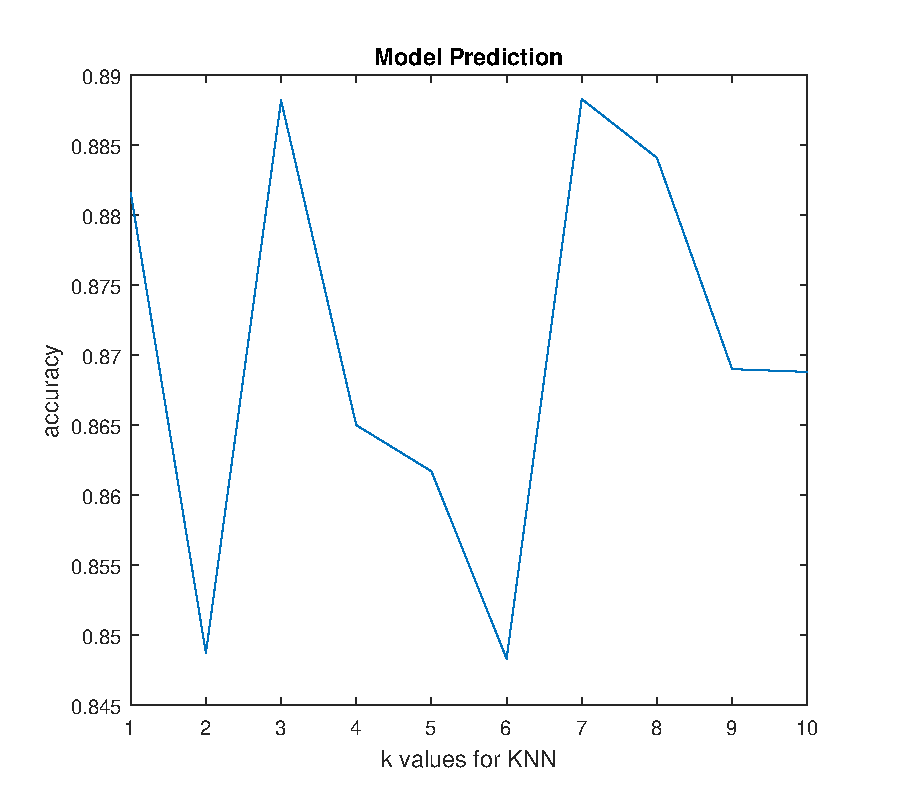
\includegraphics[scale=0.65]{acc2D3k.eps}
  \caption{Plot of the accuracy for the 2D of our model with a feature accuracy of 91\% and model accuracy with k values from 1 to 10 for KNN}\label{fig:Features2d3k}
\end{figure}

It should be noted that there is a possibility that for $k=3$ the model could be biased because we have chosen features for $k=3$ as seen in table \ref{tab:Features2d3k}. As seen in figure \ref{fig:Features2d3k} the model has the highest accuracy for both $k=3$ and $k=7$ which means that for nearest neighbours 3 and 7 we get of 88.83\% which is slightly higher than the naive feature selection, but it should be noted the this is done for 2D and the naive is 3D. So lets compare the 3D SFS with the naive selection which is more fair.

With the 3D SFS it seems that $k=1$ is in favor with the highest feature accuracy as seen in tab \ref{tab:Features3d1k} with a whole of 10 features before the feature accuracy does not improve any more

\begin{table}[H]
  \centering
    \begin{tabular}{|r|r|r|r|r|}
    \hline
          & Accuracy & Offset & Metric & Distance \\
    \hline
    Feature 1 & 0.82  & 10    & 13    & 2 \\
    \hline
    Feature 2 & 0.86  & 4     & 13    & 5 \\
    \hline
    Feature 3 & 0.87  & 12    & 13    & 7 \\
    \hline
    Feature 4 & 0.87  & 12    & 8     & 7 \\
    \hline
    Feature 5 & 0.87  & 5     & 8     & 8 \\
    \hline
    Feature 6 & 0.88  & 10    & 8     & 7 \\
    \hline
    Feature 7 & 0.92  & 2     & 13    & 6 \\
    \hline
    Feature 8 & 0.93  & 6     & 8     & 10 \\
    \hline
    Feature 9 & 0.94  & 8     & 13    & 7 \\
    \hline
    Feature 10 & \textbf{0.95}  & 3     & 10    & 7 \\
    \hline
    Feature 11 & 0.95  & 4     & 1     & 3 \\
    \hline
    \end{tabular}%
  \caption{Eleven features shown for $k=1$}\label{tab:Features3d1k}%
\end{table}%

With are feature accuracy of 95\% with 10 features needed, we are now interested to see what the model can predict.

\begin{figure}[H]
  \centering
  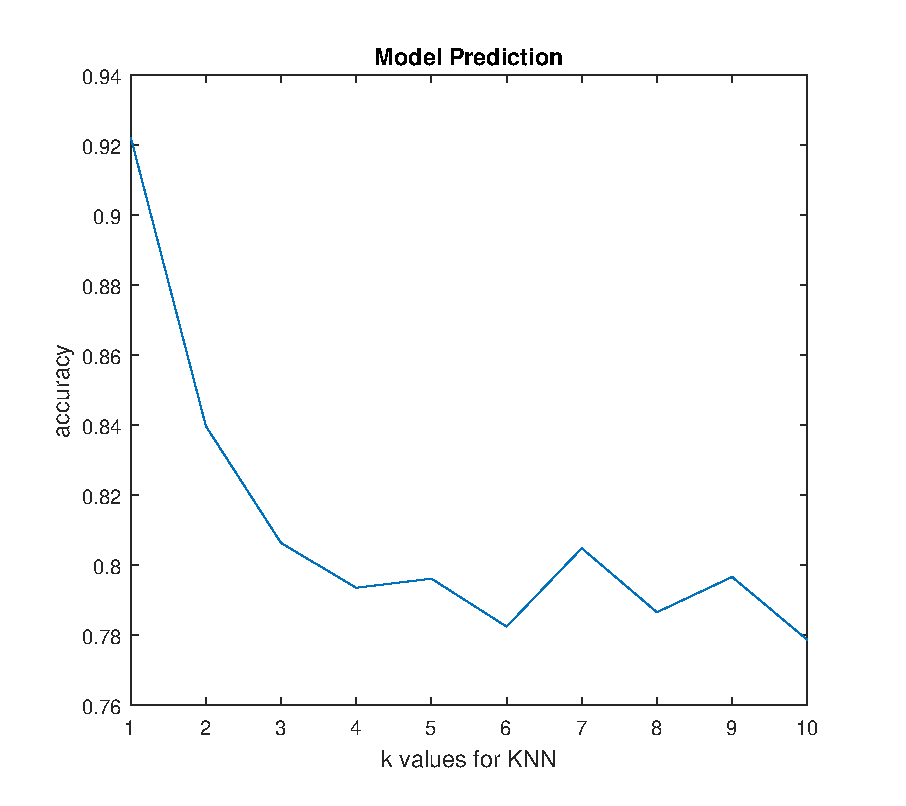
\includegraphics[scale=0.65]{acc3D1k.eps}
  \caption{Plot of the accuracy for the 3D of our model with a feature accuracy of 95\% and model accuracy with k values from 1 to 10 for KNN}\label{fig:Features3d1k}
\end{figure}

As it is possible to see in figure \ref{fig:Features3d1k} the accuracy is 92.23\% for $k=1$, which can be biased. This accuracy is also a lot higher than what we got with the naive feature selection. It is shown in figure \ref{fig:Features3d1k} that when we expand our search to more than 1 nearest neighbour that the accuracy falls drastically.

\section{Overfitting}
In the forward feature selection algorithm we attempt to avoid overfitting by creating a 10-fold cross validation, but in order to avoid overfitting more successfully it would be a better idea to keep randomizing the folds, our implementation creates the folds firstly and then run the entire feature selection without shuffling the folds. Since we do not reshuffle the data we are making our feature selection biased towards this specific partition. We can see this bias by running a test using our forward feature selection on 60 patients, and using the last 40 to test.
Running the feature selection on the data gained from using three-dimensional GLCMs with erosion and normalizing, and using 10-fold cross validation, with 6 (3 Control and 3 AD) in each folds. The feature selection results in an accuracy of 98\% on k-nn model, with k = 1. However testing this model on the remaining 40 patients using 10-fold cross validation with 4(2 Control and 2 AD) in each fold, the accuracy is instead 80\% and the best k value for the knn model is instead  k = 3 or k = 5.
Running the same test on the two-dimensional we get an accuracy of 95\% with optimal k = 1 or k = 3, where each k does not select the same features but do have some overlap. The model created using the features from the first k gives us an accuracy of 82.50\% when validating with the test set and optimal k = 9, the other model has an accuracy of 80\%, obtained for each of k ={2,3,5,7}.
This biased could have been prevented by shuffled the data a significant amount times, and for each sample run a 10-fold cross-validation to test each feature, this however would be very computational heavy, as each feature selection currently takes roughly 30 minutes to run.




Start med at snakke om Normalized Erode

Sammenligne med 2D og 3D

Hvorfor er 2D bedre end 3D eller omvendt. hvilke angles er i virkeligheden forskellige?



Hvorfor har vi valgt de algoritmer vi har

Hvorfor, hvorfor ikke normalisere.

Diskutere Erode vs Ikke Erode

Left Hippo vs right Hippo


Plots af breaks i accuracy og ændring i k for knn 